\documentclass{standalone}
\usepackage{tikz}
\usetikzlibrary{patterns}
\usetikzlibrary{positioning}
\usetikzlibrary{patterns, positioning}
\usetikzlibrary{shapes.misc}
\usepackage[outline]{contour}
\contourlength{1.5pt} 
\usepackage[sfdefault]{ClearSans}

\begin{document}
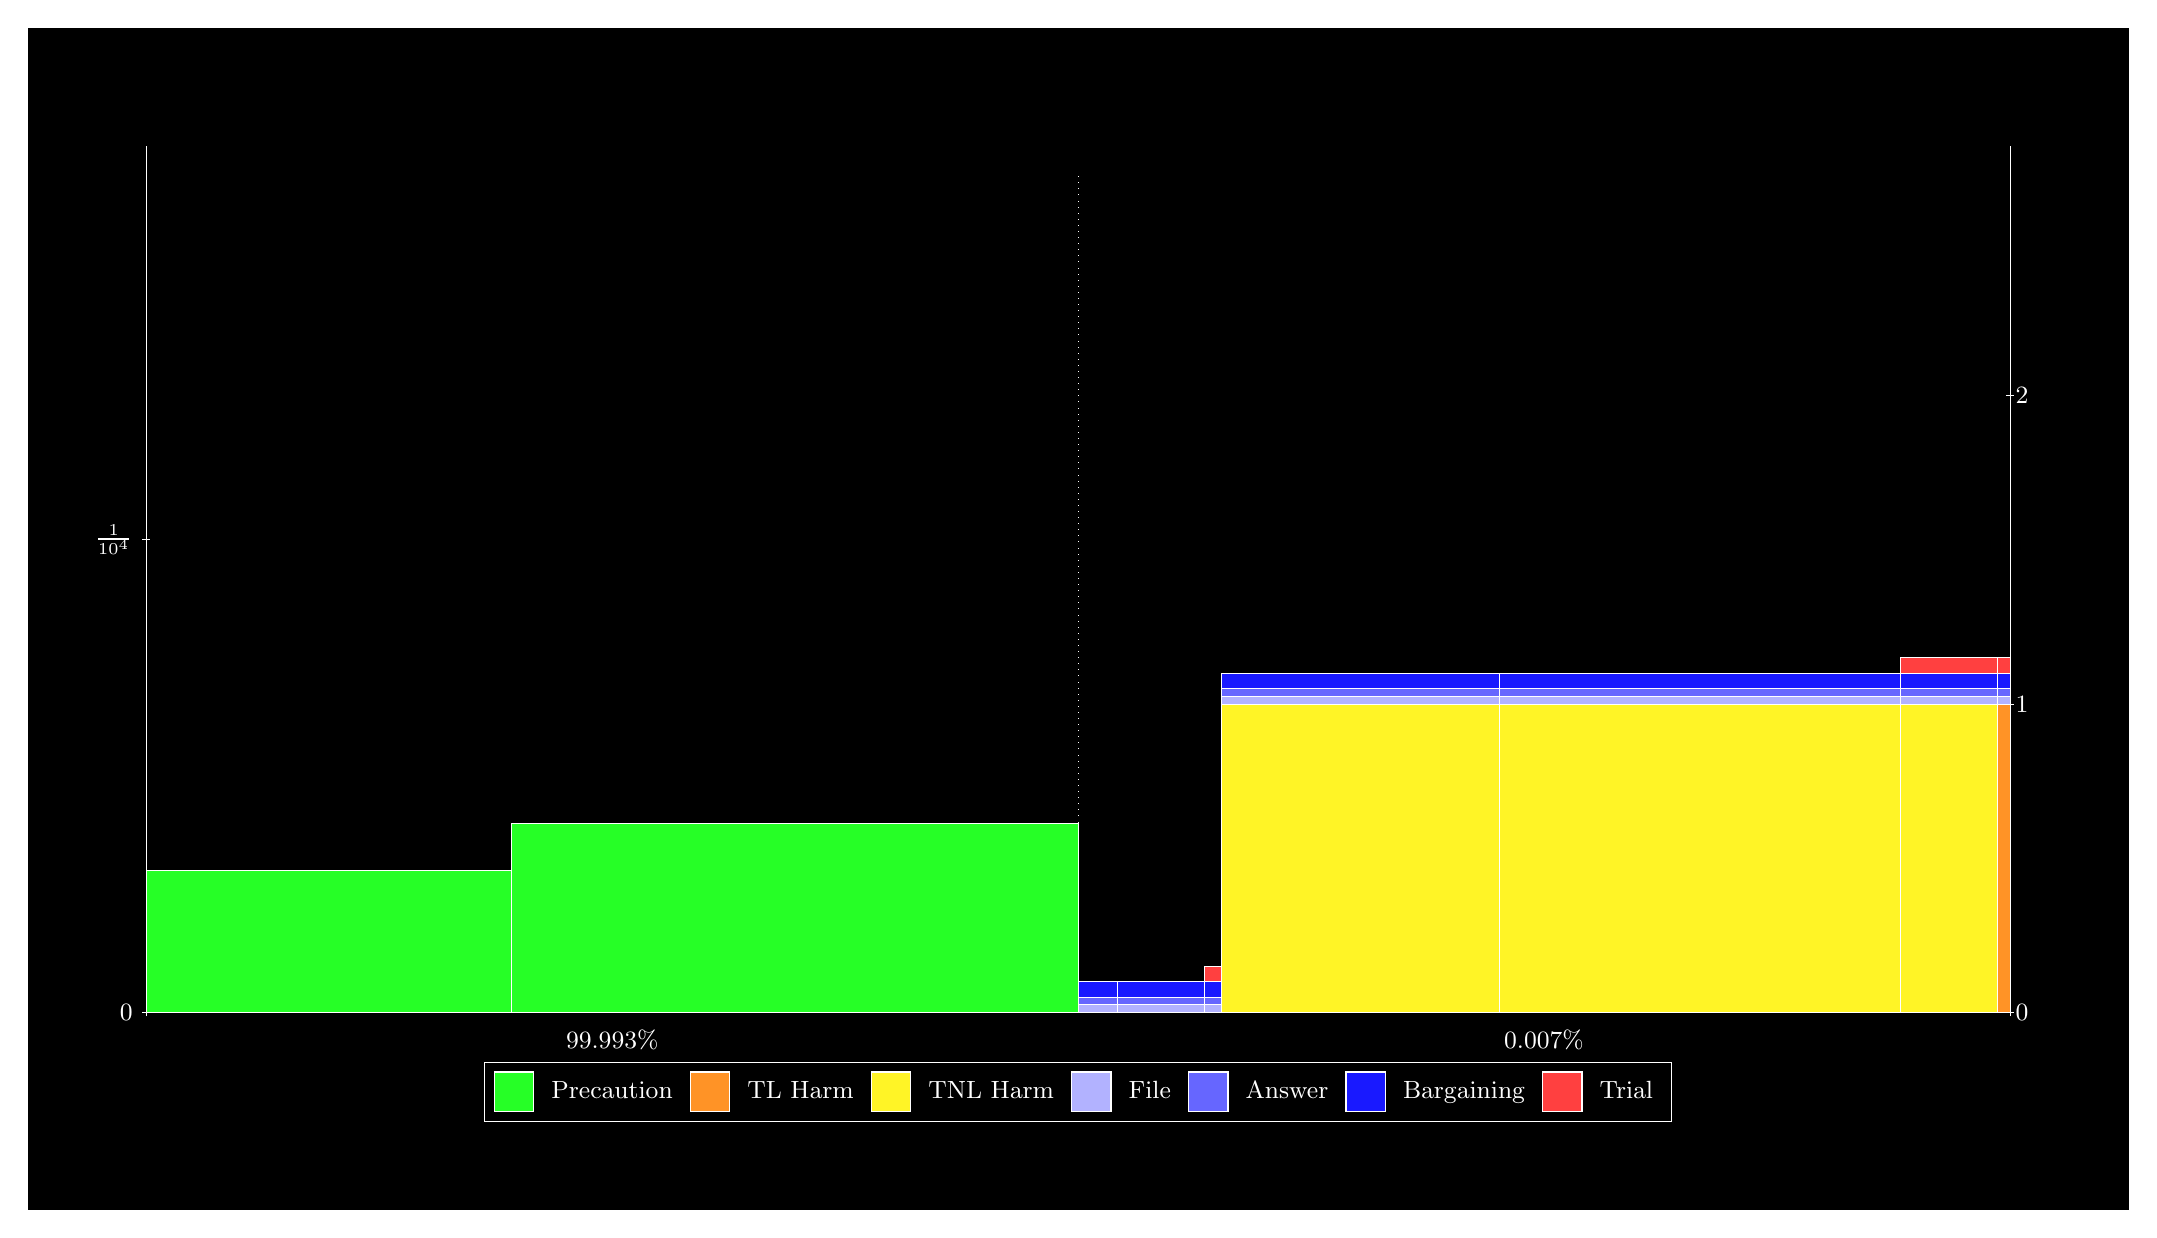
\begin{tikzpicture}
\draw[fill=black] (0,0) rectangle (26.667,15);
\draw[fill=green!85,draw=white,very thin] (1.5,2.5) rectangle (6.1372,4.3027);
\draw[fill=green!85,draw=white,very thin] (6.1372,2.5) rectangle (13.333,4.9036);
\draw[fill=green!85,draw=white,very thin] (13.333,2.5) rectangle (13.828,2.5001);
\draw[fill=blue!30,draw=white,very thin] (13.333,2.5001) rectangle (13.828,2.5981);
\draw[fill=blue!60,draw=white,very thin] (13.333,2.5981) rectangle (13.828,2.696);
\draw[fill=blue!90,draw=white,very thin] (13.333,2.696) rectangle (13.828,2.8919);
\draw[fill=green!85,draw=white,very thin] (13.828,2.5) rectangle (14.932,2.5002);
\draw[fill=blue!30,draw=white,very thin] (13.828,2.5002) rectangle (14.932,2.5981);
\draw[fill=blue!60,draw=white,very thin] (13.828,2.5981) rectangle (14.932,2.696);
\draw[fill=blue!90,draw=white,very thin] (13.828,2.696) rectangle (14.932,2.8919);
\draw[fill=green!85,draw=white,very thin] (14.932,2.5) rectangle (15.148,2.5001);
\draw[fill=blue!30,draw=white,very thin] (14.932,2.5001) rectangle (15.148,2.5981);
\draw[fill=blue!60,draw=white,very thin] (14.932,2.5981) rectangle (15.148,2.696);
\draw[fill=blue!90,draw=white,very thin] (14.932,2.696) rectangle (15.148,2.8919);
\draw[fill=red!75,draw=white,very thin] (14.932,2.8919) rectangle (15.148,3.0878);
\draw[fill=green!85,draw=white,very thin] (15.148,2.5) rectangle (18.679,2.5001);
\draw[fill=yellow!85,draw=white,very thin] (15.148,2.5001) rectangle (18.679,6.4178);
\draw[fill=blue!30,draw=white,very thin] (15.148,6.4178) rectangle (18.679,6.5157);
\draw[fill=blue!60,draw=white,very thin] (15.148,6.5157) rectangle (18.679,6.6137);
\draw[fill=blue!90,draw=white,very thin] (15.148,6.6137) rectangle (18.679,6.8096);
\draw[fill=green!85,draw=white,very thin] (18.679,2.5) rectangle (18.688,2.5001);
\draw[fill=orange!85,draw=white,very thin] (18.679,2.5001) rectangle (18.688,6.4178);
\draw[fill=blue!30,draw=white,very thin] (18.679,6.4178) rectangle (18.688,6.5157);
\draw[fill=blue!60,draw=white,very thin] (18.679,6.5157) rectangle (18.688,6.6137);
\draw[fill=blue!90,draw=white,very thin] (18.679,6.6137) rectangle (18.688,6.8096);
\draw[fill=green!85,draw=white,very thin] (18.688,2.5) rectangle (23.781,2.5002);
\draw[fill=yellow!85,draw=white,very thin] (18.688,2.5002) rectangle (23.781,6.4178);
\draw[fill=blue!30,draw=white,very thin] (18.688,6.4178) rectangle (23.781,6.5158);
\draw[fill=blue!60,draw=white,very thin] (18.688,6.5158) rectangle (23.781,6.6137);
\draw[fill=blue!90,draw=white,very thin] (18.688,6.6137) rectangle (23.781,6.8096);
\draw[fill=green!85,draw=white,very thin] (23.781,2.5) rectangle (25.012,2.5001);
\draw[fill=yellow!85,draw=white,very thin] (23.781,2.5001) rectangle (25.012,6.4178);
\draw[fill=blue!30,draw=white,very thin] (23.781,6.4178) rectangle (25.012,6.5157);
\draw[fill=blue!60,draw=white,very thin] (23.781,6.5157) rectangle (25.012,6.6137);
\draw[fill=blue!90,draw=white,very thin] (23.781,6.6137) rectangle (25.012,6.8096);
\draw[fill=red!75,draw=white,very thin] (23.781,6.8096) rectangle (25.012,7.0054);
\draw[fill=green!85,draw=white,very thin] (25.012,2.5) rectangle (25.167,2.5001);
\draw[fill=orange!85,draw=white,very thin] (25.012,2.5001) rectangle (25.167,6.4178);
\draw[fill=blue!30,draw=white,very thin] (25.012,6.4178) rectangle (25.167,6.5157);
\draw[fill=blue!60,draw=white,very thin] (25.012,6.5157) rectangle (25.167,6.6137);
\draw[fill=blue!90,draw=white,very thin] (25.012,6.6137) rectangle (25.167,6.8096);
\draw[fill=red!75,draw=white,very thin] (25.012,6.8096) rectangle (25.167,7.0054);
\draw[white,very thin] (1.5,2.5) -- (1.5,13.5);
\draw[white,very thin] (1.45,2.5) -- (1.55,2.5);
\node[font=\small,text=white, anchor=east] at (1.45, 2.5) {0};
\draw[white,very thin] (1.45,8.509) -- (1.55,8.509);
\node[font=\small,text=white, anchor=east] at (1.45, 8.509) {$\frac{1}{10^{4}}$};

\draw[white,dotted,very thin] (13.333,2.83) -- (13.333,13.17);
\draw[white,very thin] (25.167,2.5) -- (25.167,13.5);
\draw[white,very thin] (25.117,2.5) -- (25.217,2.5);
\node[font=\small,text=white, anchor=west] at (25.117, 2.5) {0};
\draw[white,very thin] (25.117,6.4177) -- (25.217,6.4177);
\node[font=\small,text=white, anchor=west] at (25.117, 6.4177) {1};
\draw[white,very thin] (25.117,10.335) -- (25.217,10.335);
\node[font=\small,text=white, anchor=west] at (25.117, 10.335) {2};

\draw[white,very thin] (1.5,2.5) -- (25.167,2.5);
\draw[white,very thin] (1.5,2.45) -- (1.5,2.55);
\node[font=\small,text=white, anchor=north] at (1.5, 2.45) {};
\draw[white,very thin] (25.167,2.45) -- (25.167,2.55);
\node[font=\small,text=white, anchor=north] at (25.167, 2.45) {};

\node[font=\small,text=white,anchor=south] at (7.4167, 1.9) {99.993\%};
\node[font=\small,text=white,anchor=south] at (19.25, 1.9) {0.007\%};
\draw (13.3333,2.5) node (B) {};
\begin{scope}[align=center]
\matrix[scale=0.5,draw=white,below=0.5cm of B,nodes={draw},column sep=0.1cm]{
\node[rectangle,draw,minimum width=0.5cm,minimum height=0.5cm,fill=green!85]{}; & \node[draw=none,font=\small,text=white]{Precaution}; &
\node[rectangle,draw,minimum width=0.5cm,minimum height=0.5cm,fill=orange!85]{}; & \node[draw=none,font=\small,text=white]{TL Harm}; &
\node[rectangle,draw,minimum width=0.5cm,minimum height=0.5cm,fill=yellow!85]{}; & \node[draw=none,font=\small,text=white]{TNL Harm}; &
\node[rectangle,draw,minimum width=0.5cm,minimum height=0.5cm,fill=blue!30]{}; & \node[draw=none,font=\small,text=white]{File}; &
\node[rectangle,draw,minimum width=0.5cm,minimum height=0.5cm,fill=blue!60]{}; & \node[draw=none,font=\small,text=white]{Answer}; &
\node[rectangle,draw,minimum width=0.5cm,minimum height=0.5cm,fill=blue!90]{}; & \node[draw=none,font=\small,text=white]{Bargaining}; &
\node[rectangle,draw,minimum width=0.5cm,minimum height=0.5cm,fill=red!75]{}; & \node[draw=none,font=\small,text=white]{Trial}; \\\\
};\end{scope}

\end{tikzpicture}
\end{document}